\documentclass[10pt,a4paper,twocolumn]{article}
\usepackage[utf8]{inputenc}
\usepackage{amsmath}
\usepackage{amsfonts}
\usepackage{amssymb}
\usepackage{graphicx}
\usepackage{hyperref}
\usepackage{listings}
\usepackage{float}
\usepackage[dutch]{babel}
\usepackage{pgfplots}
\author{Ruben Van Assche}
\graphicspath{ {../plots/} }
\lstset{
  basicstyle=\ttfamily,
  columns=fullflexible,
  breaklines=true
}
\title{Stelsels Lineaire Vergelijkingen - Oefening 5}
\date{\today}
\begin{document}
\maketitle
\section{Software}
Doorheen deze opgave heb ik gebruik gemaakt van GSL\footnote{\url{https://www.gnu.org/software/gsl/}}. Alle functies in deze opgave gebruikt komen dan ook uit de \texttt{\detokenize{gsl_linalg}} workspace, de \texttt{\detokenize{gsl_sf}} workspace en natuurlijk de functies voor matrices(\texttt{\detokenize{gsl_matrix}}) en vector.(\texttt{\detokenize{gsl_vector}}).
\newline
\newline
Informatie over het compileren en runnen van het programma kan gevonden worden in \texttt{\detokenize{README.md}}.
\section{Opgave}
Het doel van deze opgave was de berekening van het volgende benchmark probleem:
$$\sum^{n}_{j = 1}a_{ij}x_{j} = \begin{pmatrix}
n + i - 1\\ 
i
\end{pmatrix} \qquad  i = 1,\hdots,n$$
$$a_{ij} = \begin{pmatrix}
i + j - 2\\
j - 1
\end{pmatrix} \qquad  x_{j}= 1$$
Hierbij moet een schatting van het conditiegetal gemaakt worden voor de matrix A waarbij $n = 3,6,9,12$. Het stelsel moet voor dezelfde $n$ waarden opgelost worden in dubbele precisie($\frac{1}{2}ULP = 2^{-53}$) en voor deze berekening moet het residu en de error vector berekend worden.
\section{De matrix A opstellen}
De opgave vereist een beperkte kennis van combinatoriek want in feite is matrix A een Pascal matrix:
$$
\begin{bmatrix}
1 & 1  & 1 \\ 
1 & 2 & 3\\ 
1 & 3 & 6
\end{bmatrix}
$$
Om deze te bereken wordt er gebruik gemaakt van een combinatie:
$$
\begin{pmatrix}
n\\ 
k
\end{pmatrix} = \frac{n!}{k!(n-k)!}
$$
Deze komen voor het voorschrift van het benchmark probleem en worden d.m.v. volgende code opgelost:
\begin{lstlisting}[language=C++]
double combinate(const unsigned int n, const unsigned int k){
    return ( gsl_sf_fact(n) )/(gsl_sf_fact(k) * gsl_sf_fact(n - k));
}
\end{lstlisting}
Deze code implementeert de gegeven wiskundige definitie van een combinatie d.m.v. \texttt{\detokenize{gsl_sf_fact}} voor het berekenen van faculteiten.
\newline
\newline
Het opstellen van de  matrices A voor verschillende waarden $n$ kan nu makkelijk gebeuren.
\subsection{n = 3}
$$
\begin{bmatrix}
1 & 1  & 1 \\ 
1 & 2 & 3\\ 
1 & 3 & 6
\end{bmatrix}
$$
\subsection{n = 6}
$$
\begin{bmatrix}
1 & 1 & 1 & 1 & 1 & 1 \\
1 & 2 & 3 & 4 & 5 & 6 \\
1 & 3 & 6 & 10 & 15 & 21 \\
1 & 4 & 10 & 20 & 35 & 56 \\
1 & 5 & 15 & 35 & 70 & 126 \\
1 & 6 & 21 & 56 & 126 & 252 \\
\end{bmatrix}
$$
\subsection{n = 9}
$$
\begin{bmatrix}
1 & 1 & 1 & 1 & 1 & 1 & 1 & 1 & 1 \\
1 & 2 & 3 & 4 & 5 & 6 & 7 & 8 & 9 \\
1 & 3 & 6 & 10 & 15 & 21 & 28 & 36 & 45 \\
1 & 4 & 10 & 20 & 35 & 56 & 84 & 120 & 165 \\
1 & 5 & 15 & 35 & 70 & 126 & 210 & 330 & 495 \\
1 & 6 & 21 & 56 & 126 & 252 & 462 & 792 & 1287 \\
1 & 7 & 28 & 84 & 210 & 462 & 924 & 1716 & 3003 \\
1 & 8 & 36 & 120 & 330 & 792 & 1716 & 3432 & 6435 \\
1 & 9 & 45 & 165 & 495 & 1287 & 3003 & 6435 & 1.287e+04 \\
\end{bmatrix}
$$
\subsection{n = 12}
\setcounter{MaxMatrixCols}{12}
$$
\begin{bmatrix}
1 & 1 & 1 & 1 & 1 & 1 & 1 & 1 & 1 & 1 & 1 & 1 \\
1 & 2 & 3 & 4 & 5 & 6 & 7 & 8 & 9 & 10 & 11 & 12 \\
1 & 3 & 6 & 10 & 15 & 21 & 28 & 36 & 45 & 55 & 66 & 78 \\
1 & 4 & 10 & 20 & 35 & 56 & 84 & 120 & 165 & 220 & 286 & 364 \\
1 & 5 & 15 & 35 & 70 & 126 & 210 & 330 & 495 & 715 & 1001 & 1365 \\
1 & 6 & 21 & 56 & 126 & 252 & 462 & 792 & 1287 & 2002 & 3003 & 4368 \\
1 & 7 & 28 & 84 & 210 & 462 & 924 & 1716 & 3003 & 5005 & 8008 & 1.238e+04 \\
1 & 8 & 36 & 120 & 330 & 792 & 1716 & 3432 & 6435 & 1.144e+04 & 1.945e+04 & 3.182e+04 \\
1 & 9 & 45 & 165 & 495 & 1287 & 3003 & 6435 & 1.287e+04 & 2.431e+04 & 4.376e+04 & 7.558e+04 \\
1 & 10 & 55 & 220 & 715 & 2002 & 5005 & 1.144e+04 & 2.431e+04 & 4.862e+04 & 9.238e+04 & 1.68e+05 \\
1 & 11 & 66 & 286 & 1001 & 3003 & 8008 & 1.945e+04 & 4.376e+04 & 9.238e+04 & 1.848e+05 & 3.527e+05 \\
1 & 12 & 78 & 364 & 1365 & 4368 & 1.238e+04 & 3.182e+04 & 7.558e+04 & 1.68e+05 & 3.527e+05 & 7.054e+05 \\
\end{bmatrix}
$$
\clearpage
\section{Conditiegetal}
Het conditiegetal geeft aan of een matrix(in deze opgave de matrix A) goed of slecht geconditioneerd is. Het meet dus hoe gevoelig het antwoord is aan storingen in de input data en aan afrondingsfouten gemaakt doorheen het oplossen van de matrix. Dit zien we aan volgende definitie: 
$$\frac{\left \| \delta{x} \right \|}{\left \| x \right \|} < \kappa(A)\frac{\left \| \delta{b} \right \|}{\left \| b \right \|} $$
Hierbij is $\frac{\left \| \delta{b} \right \|}{\left \| b \right \|}$ de relatieve wijziging in de rechterkant van het stelsel $Ax = b$ en $\frac{\left \| \delta{x} \right \|}{\left \| x \right \|}$ de relatieve wijziging in de oplossing van het stelsel. Wat opvalt is dat het conditiegetal $\kappa(A)$ een vergrotingsfactor is voor relatieve wijzigingen aan de rechterkant van het stelsel die vergrotingen van $\kappa(A)$ kan veroorzaken in de oplossing van het stelsel.
\newline
\newline
Een groot conditiegetal kan er dus voor zorgen dat de fout in de oplossing van het stelsel gigantisch groot wordt!
\subsection{Berekening}
Voor het berekenen van het conditiegetal wordt er gebruik gemaakt van een singuliere waarden decompositie(in GSL : \texttt{\detokenize{gsl_linalg_SV_decomp}}). Deze singuliere waarden $\sigma_{i}$ met $i = 1,\hdots,n$ worden gebruikt om het conditiegetal te berekenen via volgende methode : 
$$\kappa(A) = \frac{max(\sigma_{i})}{min(\sigma_{i})} \qquad i = 1,\hdots,n$$
De code voor het berekenen van het conditiegetal is te vinden in \texttt{\detokenize{Utils.h}}.
\subsection{Resultaten}
$$
 \begin{tabular}{ l | r }
   \textbf{n} & \textbf{Conditiegetal} \\ \hline
   3 & 61.98 \\
   6 & 1.108e+05 \\
   12 & 2.908e+08 \\
   15 & 8.764e+11 \\
\end{tabular}
$$
Wat opvalt is dat naarmate de $n$ groter wordt, het conditiegetal exponentieel groter wordt, dit zal grote gevolgen hebben in latere delen van deze opgave!
\newline
Dit zien we als we een grafiek maken van de conditiegetallen(let op er wordt hier gebruik gemaakt van een logaritmische schaal):
\begin{figure}[H]
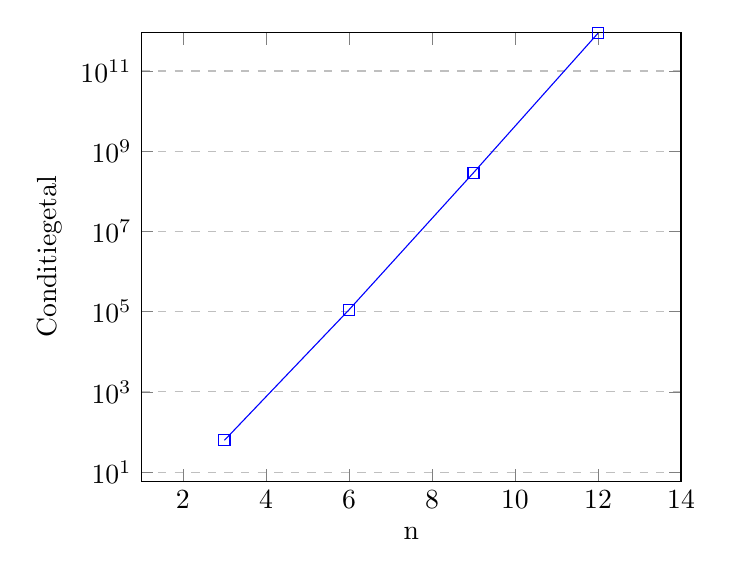
\begin{tikzpicture}
\begin{axis}[
    xlabel={n},
    ylabel={Conditiegetal},
    ymode=log,
    xmin=1, xmax=14,
    ymin=0, ymax= 9e+11,
    legend pos=north west,
    ymajorgrids=true,
    grid style=dashed,
]
 
\addplot[
    color=blue,
    mark=square,
    ]
    coordinates {
    (3,61.98)(6, 1.108e+05)(9,2.908e+08)(12,8.764e+11)
    };
 
\end{axis}
\end{tikzpicture}
\label{fig:conditiegetalgrafiek}
\caption{Conditiegetallen voor verschillende n}
\end{figure}
\section{Oplossen stelsel}
Voor het oplossen van het stelsel wordt er gebruik gemaakt van GEPP, de functies hiervoor in GSL zijn \texttt{\detokenize{gsl_linalg_LU_decomp}} en \texttt{\detokenize{gsl_linalg_LU_solve}}. Hiermee lossen we het stelsel $Ax = b$ met $n = 3,6,9,12$ op.
\newline
\newline
In de opgave wordt gevraagd om het stelsel in dubbele precisie($\frac{1}{2}ULP = 2^{-53}$) op te lossen. In C/C++ betekent dit het gebruik van het double type. Maar deze kan per machine verschillend zijn. Volgende checkt de precisie van het double type op de machine waar het programma draait:
\begin{lstlisting}
    std::cout << "ULP double : " << std::numeric_limits<double>::epsilon() << std::endl;
    std::cout << "ULP required : " << pow(2, -52) << std::endl;
\end{lstlisting}
Wanneer beide functies hetzelfde resultaat opleveren hebben we double precisie zoals gevraagd.
\newline
\newline
GSL gebruikt voor haar implementatie van matrices en vectoren ook het double type, dit is zeer belangrijk gezien GEPP geïmplementeerd door GSL gebruik maakt van deze structuren.
\subsection{Het Residu en de error vector}
Om meer te kunnen zeggen over de correctheid van de oplossing berekenen we voor elke oplossing ook nog het residu:
$$r = y - A\tilde{x}$$
en de error vector : 
$$e = x^{\star} - \tilde{x}$$
Hierbij is $\tilde{x}$ de berekende oplossing en $x^{\star}$ de exacte wiskundige oplossing.
\subsection{Resultaten}
\subsubsection{n = 3}
 \begin{tabular}{ l | c | r }
   \textbf{x} & \textbf{residu} & \textbf{error} \\ \hline
   -12.01 & 9.598 & 13.01 \\
   0.8165 & 5.432 & 0.1835 \\
   0.008774 & 10.01 & 0.9912 \\
\end{tabular}
\subsubsection{n = 6}
 \begin{tabular}{ l | c | r }
   \textbf{x} & \textbf{residu} & \textbf{error} \\ \hline
   -544 & 58.03 & 545 \\
   -22.1 & 37.07 & 23.1 \\
   2.212 & 54.47 & -1.212 \\
   -0.1813 & 125.9 & 1.181 \\
   0.00149 & 252 & 0.9985 \\
   -8.086e-07 & 462 & 1\\
\end{tabular}
\subsubsection{n = 9}
 \begin{tabular}{ l | c | r }
   \textbf{x} & \textbf{residu} & \textbf{error} \\ \hline
   -2.843e+04  & 433.7 & 2.843e+04\\
   -745.1 & 207 & 746.1\\
   -45.54 & 204.2 & 46.54\\
   5.018 & 491.9 & -4.018\\
   0.7201 & 1287 & 0.2799\\
   0.03267 & 3003 & 0.9673\\
   -0.000223 & 6435 & 1\\
   2.939e-07 & 1.287e+04 & 1\\
   4.364e-11 & 2.431e+04 & 1\\
\end{tabular}
\subsubsection{n = 12}
 \begin{tabular}{ l | c | r }
   \textbf{x} & \textbf{residu} & \textbf{error} \\ \hline
-1.576e+06 &  3.051e+04 & 1.576e+06\\
-3.05e+04 & 7621 & 3.05e+04\\
-1317 & 1530 & 1318 \\
96.84 & 1319 & -95.84 \\
-11.04 & 4372 & 12.04\\
1.795 & 1.238e+04 & -0.795 \\
0.2083 & 3.182e+04 & 0.7917 \\
-0.005095 & 7.558e+04 & 1.005 \\
3.222e-05 & 1.68e+05 & 1 \\
6.252e-08 & 3.527e+05 & 1 \\
-2.968e-11 & 7.054e+05 & 1 \\
5.3e-12 & 1.352e+06 & 1 \\
\end{tabular}
\section{Bespreking Resultaten}
Als laatste deel van deze opgave bekijken we de resultaten en de relatie ertussen. Eerst kijken we naar het conditiegetal, zoals gezien op de plot in ~\ref{fig:conditiegetalgrafiek} zien we dat naarmate $n$ groter wordt het conditiegetal exponentieel groter wordt. Dit heeft een effect op de residu en error vectoren: de waarden in deze vectoren worden groter.
\\
Om dit te staven heb ik voor elke residu en error vector de euclidische norm berekend d.m.v. \texttt{\detokenize{gsl_blas_dnrm2}}:
\\
\\
 \begin{tabular}{ l | c | r }
   \textbf{n} & \textbf{residu} & \textbf{error} \\ \hline
   3 & 14.89 & 13.05 \\
   6 & 548.2 & 545.5 \\
   9 & 2.845e+04 & 2.844e+04 \\
   12 & 1.577e+06 & 1.576e+06 \\
\end{tabular}
\\
\\
Wanneer we deze waarden plotten op een grafiek bekomen we een gelijkaardige grafiek als in ~\ref{fig:conditiegetalgrafiek}:
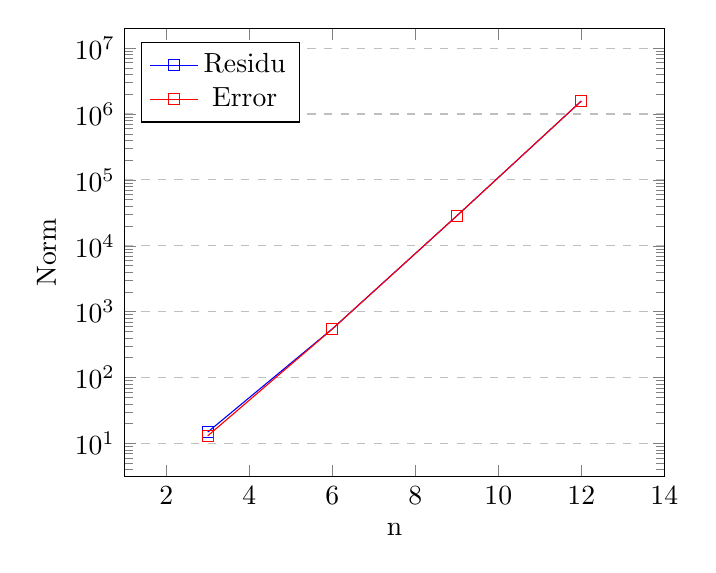
\begin{tikzpicture}
\begin{axis}[
    xlabel={n},
    ylabel={Norm},
    ymode=log,
    xmin=1, xmax=14,
    ymin=0, ymax= 2e+7,
    legend pos=north west,
    ymajorgrids=true,
    grid style=dashed,
]
 
\addplot[
    color=blue,
    mark=square,
    ]
    coordinates {
    (3,14.89)(6, 548.2)(9,2.845e+04)(12,1.577e+06)
    };
 \addplot[
    color=red,
    mark=square,
    ]
    coordinates {
    (3,13.05)(6, 545.5)(9,2.844e+04)(12, 1.576e+06)
    };
    \legend{Residu, Error}
\end{axis}
\end{tikzpicture} 
\\
Dit is logisch! Zoals al eerder aangehaald zal naarmate het conditiegetal groter is de fout in de oplossing groter worden. Kijken we naar de x vector voor elke $n$ dan zien we dat deze zelfs al bij een kleine $n = 3$ een zeer grote afwijking van de wiskundig berekende oplossing waarbij elke waarde in de vector 1 is. Dit is dan ook de waarde die we zien in de error vector. Deze geeft aan in hoeverre de berekende oplossing afwijkt van de wiskundige oplossing. 
\\
\\
De grootte van het residu volgt naarmate dat $n$ groter wordt de grootte van de error vector. Dit komt omdat het residu weergeeft in hoeverre de oplossing de lineaire condities in $Ax = b$ goed volgt. Gezien de waarden in de $x$ vector voor elke $n$ zo goed als niet in de buurt van 1 liggen, zal bij het oplossen van het stelsel $Ax$ nooit een vector verkregen worden die in de buurt ligt van vector $b$. Met als gevolg dat het residu ook zeer groot wordt.
\subsection{Samengevat}
Er is een zeer duidelijke relatie is tussen al deze grootheden berekend in de opgave. Een slecht geconditioneerde matrix A zal zorgen voor een groot conditiegetal, wanneer dan het stelsel $Ax = b$ wordt opgelost zal door het grote conditiegetal de vector $x$ niet in de buurt komen van haar wiskundig berekende versie. Dit zorgt er dan weer voor dat de error vector zeer grote waarden bevat. De waarden in de residu vector zullen dan ook groot worden omdat bij het oplossen van het stelsel $Ax$ met de berekende vector $x$ de uitkomst nooit $b$ zal benaderen.
\end{document}